\chapter{Network}
\section{Proprietà dei grafi}
Quando le dimensioni dei grafi iniziano a crescere risulta difficile
rappresentarli in modo chiaro e comprensibile. Per questo motivo, quando si
lavora con grafi di grandi dimensioni, essi vengono rappresentati tramite
delle proprietà che ne descrivono la struttura.

Tra le proprietà più importanti troviamo:
\begin{itemize}
    \item \textbf{Lunghezza media dei cammini}: indica la lunghezza media dei
          cammini tra due nodi.
    \item \textbf{Diametro}: indica la lunghezza del cammino più lungo tra due
          nodi.
    \item \textbf{Grado di un nodo}: indica il numero di archi che partono o
          arrivano ad un nodo.
    \item \textbf{Coefficienti di clustering}: indicano la presenza di nodi
          vicini tra loro.
    \item \textbf{Centralità}: indica l'importanza di un nodo all'interno del
          grafo.
\end{itemize}
\subsection{Grado di un nodo}
\begin{definizione}[\textbf{Grado di un nodo}]
    Il \textbf{grado di un nodo} è il numero di archi che partono o arrivano ad
    un nodo. Nel caso di grafi diretti si parla di \textbf{grado uscente} o
    \textbf{out degree} e \textbf{grado entrante} o \textbf{in degree}.
\end{definizione}

Se si considera un grafo rappresentato attraverso una matrice di adiacenza, il
grado di un nodo può essere calcolato sommando i valori della riga o della
colonna corrispondente al nodo in questione. Nello specifico, se si considera
un grafo orientato, il grado uscente di un nodo corrisponde alla somma dei
valori della riga corrispondente al nodo, mentre il grado entrante corrisponde
alla somma dei valori della colonna corrispondente al nodo.

Più in generale possiamo riassumere il calcolo del grado di un nodo come segue:
\begin{equation}
    \text{Outdegree}(i) = \sum_{j=1}^{n} A_{ij} \quad \text{e} \quad
    \text{Indegree}(i) = \sum_{j=1}^{n} A_{ji}
\end{equation}
dove $A_{ij}$ è l'elemento della matrice di adiacenza corrispondente al nodo
$i$ e $j$. Nel caso di grafi non orientati, il grado di un nodo corrisponde
alla somma dei valori della riga o della colonna corrispondente al nodo in
questione.

Il grado di un nodo rappresenta una misura locale del grafo, nel caso in cui
si voglia ottenere una misura globale del grafo si può calcolare il grado
medio dei nodi. Tale misura può essere calcolata come segue:
\begin{equation}
    \langle k \rangle = \frac{1}{n} \sum_{i=1}^{n} \text{Grado}(i)
\end{equation}
dove $n$ rappresenta il numero di nodi del grafo. Anche in questo caso, se il
grafo è orientato dobbiamo distinguere tra grado uscente e grado entrante.
\begin{nota}
    Possiamo calcolare il grado medio anche come segue:
    \begin{itemize}
        \item Nel caso di grafi non orientati:
              \begin{equation}
                  \langle k \rangle = \frac{2E}{n}
              \end{equation}
              dove $E$ rappresenta il numero di archi del grafo.
        \item Nel caso di grafi orientati:
              \begin{equation}
                  \langle k \rangle = \frac{E}{n}
              \end{equation}
              dove $E$ rappresenta il numero di archi.
    \end{itemize}
\end{nota}
Una misura più rappresentativa della media dei gradi dei nodi è la \textbf{distribuzione
    dei gradi}. Possiamo definire $p(k)$ come la probabilità che un nodo abbia
grado $k$. Tale distribuzione può essere calcolata come segue:
\begin{equation}
    p(k) = \frac{n_k}{n}
\end{equation}
dove $n_k$ rappresenta il numero di nodi con grado $k$ e $n$ rappresenta il
numero totale di nodi del grafo. La distribuzione dei gradi può essere
rappresentata tramite un istogramma, in cui sull'asse delle ascisse vengono
inseriti i valori dei gradi, mentre sull'asse delle ordinate sono presenti i
valori di $p(k)$.
\begin{figure}[!ht]
    \centering
    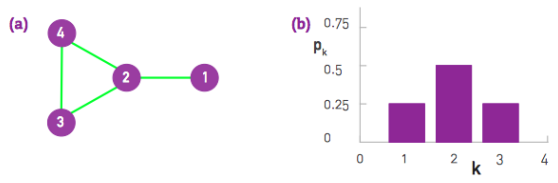
\includegraphics[width=0.7\textwidth]{./img/net/degreedist.png}
    \caption{Esempio di distribuzione dei gradi.}
    \label{fig:degree_distribution}
\end{figure}
\begin{nota}
    Questa distribuzione deve essere normalizzata, ovvero la somma di tutti i
    valori di $p(k)$ deve essere uguale a 1.
    \begin{equation*}
        \sum_{k=0}^{\infty} p(k) = 1
    \end{equation*}
\end{nota}

Il valore della distribuzione mi permette di rappresentare molti fenomeni dalla
robustezza della rete alla sua vulnerabilità.
\subsection{Cammino e distanza}
\begin{definizione}[\textbf{Cammino}]
    Un \textbf{cammino} è una sequenza di nodi in cui ciascun nodo è adiacente
    al successivo.
\end{definizione}
\begin{definizione}[\textbf{Distanza}]
    La \textbf{distanza} tra due nodi è definita come il numero minimo di archi
    che devono essere attraversati per andare da un nodo all'altro. Se i due
    nodi non sono collegati, la distanza è infinita.
\end{definizione}
Un modo semplice per calcolare la distanza tra due nodi è quello di utilizzare
l'algoritmo BFS (Breadth First Search).
\begin{definizione}[\textbf{Diametro}]
    Il diametro di un grafo è la distanza massima tra due nodi nel grafo.
\end{definizione}
\begin{definizione}[\textbf{Lunghezza media dei cammini}]
    La lunghezza media dei cammini è la media delle distanze tra tutti i nodi
    del grafo. Tale misura può essere calcolata come segue:
    \begin{equation}
        \langle d \rangle = \frac{1}{2E_{max}} \sum_{i \neq j} d_{ij}
    \end{equation}
\end{definizione}
Nei grafi non orientati, la lunghezza media dei cammini può essere calcolata
come segue:
\begin{equation}
    \langle d \rangle = \frac{1}{E_{max}} \sum_{i \neq j} d_{ij}
\end{equation}
dove $d_{ij}$ rappresenta la distanza tra i nodi $i$ e $j$ e $E_{max}$ rappresenta
il numero massimo di archi presenti nel grafo.
\subsection{Coefficienti di clustering}
\begin{definizione}[\textbf{Coefficienti di clustering}]
    I coefficienti di clustering sono una misura della presenza di nodi vicini
    tra loro. In particolare, il coefficiente di clustering di un nodo è una
    misura della probabilità che i vicini di un nodo siano collegati tra loro.
    Dato un nodo $i$ con grado $k_i$, il coefficiente di clustering locale è
    definito come segue (grafo indiretto):
    \begin{equation}
        C_i = \frac{2E_i}{k_i(k_i - 1)}
    \end{equation}
    dove $E_i$ rappresenta il numero di archi tra i vicini del nodo $i$. Se il grafo
    è diretto allora si divide per $2$ il coefficiente.
\end{definizione}

Il valore di questo coefficiente può variare tra 0 e 1. Nel caso in cui il
coefficiente sia uguale a 1, significa che tutti i vicini del nodo $i$ sono
collegati tra loro. Nel caso in cui il coefficiente sia uguale a 0, significa
che nessun vicino del nodo $i$ è collegato ad un altro vicino.

% TODO: immagine di come varia il coefficiente di clustering

Questa misura rappresenta la densità locale di un grafo. Per ottenere una
misura \textbf{globale} della densità del grafo, possiamo calcolare il \textbf{coefficiente
    di clustering medio}. Tale misura può essere calcolata come segue:
\begin{equation}
    \langle C \rangle = \frac{1}{n} \sum_{i=1}^{n} C_i
\end{equation}
dove $\langle C \rangle$ si può interpretare come la probabilità che due vicini
di un nodo, selezionato in modo casuale, siano collegati tra loro. 

La distribuzione di grado ci da informazioni in più rispetto alla media, perché
è uno stimatore distorto, sarebbe meglio la mediana però generalmente si analizza
direttamente la distribuzione di grado. Inoltre la distribuzione di grado permette 
di studiare gli hub (tutti i nodi che sono caratterizzati da un alto grado e bassa 
probabilità di occorrere nella rete molto basso).

Grafico della distribuzione delle distanze nel grafo mi mostra il diametro, la media 
e capire se sono molto presenti le distanze ampie o basse.

Il oefficiente di clustering medio permette di capire quanto sono connessi i vicini
di un nodo estratto casualmente. Il grafico del coeff. di clustering ci mostra 
le relazioni tra grado e clustering. (ex: spoke hanno un coeff. di clustering maggiore 
quindi il vicinato è molto connesso, sintomo organizzazione gerarchica).  

Con questi ragionamenti si riesce ad effettuare inferenze sul comportamento che 
si ottiene se si dovessere rimuovere un nodo.

\subsection{Centralità del grafo}
Esistono diversi criteri per determinare la rilevanza del nodo (centrale). 

Esistono diverse tipologie di centralità:
\begin{itemize}
    \item \textbf{degree} (non diretta): numero di collegamenti con i vici, coincide col grado
    ciascun nodo.
    $$C_D(i) = \sum_j x_{ij}$$
    La centralità massima per un nodo è $n-1$ e spesso si calcola la centralità di 
    grado normalizzata (divisa per la centralità massima).
    \item \textbf{degree} (diretta):
    \begin{itemize}
        \item in-degree:
        \item out-degree:
    \end{itemize}
    \item \textbf{betweeness} (centralità di ponte o collo di bottiglia): 
    $$C_B(i) = \sum_{i\ne k \ne i} \frac{g_{jk}(i)}{g_{jk}}$$
    Dove:
    \begin{itemize}
        \item $g_{ik}(i)$: corrisponde al numero di Shortest path tra $jk$ nella rete tale che 
        passa da $i$
        \item $g_{ik}$: corrisponde al numero di Shortest parth tra $jk$
    \end{itemize}
    Normalizziamo sui noti per confrontare reti con numero di nodi differenti.
    Centralità massima significa nodo con maggiore capacità di unire gruppi. Centralità $0$
    allora è un nodo posso perché non collega nessuno.
    
    Poi il coeff. di centralità viene normalizzato sul totale di tutti gli shortest 
    path nel diretto o nel non orientato
    \item \textbf{closeness}: calcola la somma di tutte le distanze tra $i$ e tutti gli altri.
    elevo alla $-1$ per renderla una centralità e non una distanza. corrisponde 
    alla misura di un vertice in merito alla sua efficienza nel comunicare l'informazionie.
    La betweeness è una misura l'efficacia di un nodo nell trasmettere un'informazione.
    \item \textbf{autovettori}: prima misura non locale di centralità. Si vuole 
    raccogliere il rapporto rispetto agli altri nodi. L'idea è se un nodo è
    importante allora tra quelli con cui è collegato ci saranno altri nodi importanti.
    % inserisci formula 
    Diverso alla centralità di grado perché non perforza un nodo è importante se 
    riceve tanti link. Si considera il grado e il ruolo dei nodi che si collegano.
    In aggiunta, un nodo con alta centralità non è necessariamente fortemente linkato
    agli altri. (valido per grafi non orientati)
    \item \textbf{pagerank} (per grafi orientati): consiste in una serie di voti
    che ogni nodo ottiene dalla rete

    matrice di transizione: mi dice la prob. che dato un nodo raggiungo un altro
    se volessi simulare la navigazione dell'utente nel web attraverso diverse pagine
    e sto moltiplicando le probabilità per ogni nodo che attraverso nella navigazione.
    Se moltiplicassi la matrice di transizione per se stessa ottengo la probabilità 
    di raggiungere un nodo da tutti. Possiamo riperlo all'infinito, ad un certo punto 
    non avremo cambiamenti ovvero quando la matrice soddisfa le proprietà di :
    \begin{itemize}
        \item stocastica: se la somma per riga è $1$. Se definisco per $\frac{1}{O}$ 
        dove $O$ ha link uscenti sarei apposto, il problema è che non tutti i nodi 
        hanno link uscenti. Risolvo % perso le robe
        \item irriducibile: se il grafo è fortemente connesso.
        \item aperiodica: un nodo viene definito come periodico se esiste un 
        ciclo che attraversa un nodo. 
    \end{itemize} 
    Per risolvere irriducibilità e aperiodicità si aggiunge un arco per ogni noto \dots
    Si ha un sistema lineare che si deve risolvere per ottenere la metrica 
    di pagerank.
    Esiste un altro algoritmo per il page rank ma non ha funzionato perché prima 
    partiva dalla creazioen del grafo che rispetta la query e poi calcola la metrica
    (troppo costoso).
\end{itemize}

Il coeff. di centralizzazione: quanta variabilità c'è tra tutte le centralità dei 
nodi, è una misura varianza della centralità di grado. Ci serve il coefficiente 
di centralità massimo di nodi del grafo ($C_D(n^\ast)$) e la centralizzazione coincide 
con la somma degli scarti della centralità tra il nodo con più centralità e tutti gli altri,
infine normalizzo per la massima somma di differenze per una rete che ha $n$ nodi.
Coeff. max ($1$) abbiamo un nodo più centrale rispetto agli altri. 

La centralità di grado non è utile per determinare la funzione di ponte (separazione 
di gruppi) (è legato la coefficiente di clustering).


